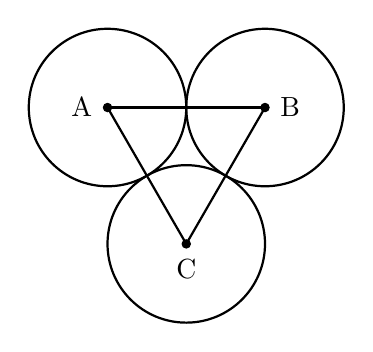
\begin{tikzpicture}[scale=1]

    % Define the centers of the circles
    % To make them touch perfectly, the distance between any two centers must be exactly 2 (sum of their radii: 1 + 1).
    % This forms an equilateral triangle with side length 2.
    % If C is at (0,0), A and B will be at y = \sqrt{3}
    \coordinate (C) at (0, 0);
    \coordinate (A) at (-1, {sqrt(3)});
    \coordinate (B) at (1, {sqrt(3)});

    % Draw the circles
    \draw[thick] (A) circle (1.0);
    \draw[thick] (B) circle (1.0);
    \draw[thick] (C) circle (1.0);

    % Draw the lines connecting the centers
    \draw[thick] (A) -- (B);
    \draw[thick] (B) -- (C);
    \draw[thick] (C) -- (A);

    % Add a small dot for each center
    \filldraw (A) circle (1.5pt);
    \filldraw (B) circle (1.5pt);
    \filldraw (C) circle (1.5pt);

    % Add labels for the points
    \node[left, xshift=-2pt] at (A) {A};
    \node[right, xshift=2pt] at (B) {B};
    \node[below, yshift=-2pt] at (C) {C};

\end{tikzpicture}